\label{33-0429}
\subsection{Permutation Groups}
Let $S$ be a set. Let $G$ be a group of permutations, $\pi$,
acting on elements of $S$. Then, $G$ is a \textbf{permutation group}.

\begin{example}1
    \[ \pi_1 = \begin{pmatrix}
        1 & 2 & 3 & 4 & 5 \\ 3 & 2 & 1 & 5 & 4
    \end{pmatrix}
        \]
    \[
        \pi_1(1) = 3, \pi_1(4) = 5, \text{etc.}
    \]
    We can write $\pi_1$ as a product of cycles, as we have 
    done in the past. 
    \[ \pi_1 = (1 \ 3) (2) (4 \ 5)\]
    This is the \textbf{cycle decomposition} of $\pi_1$. 
\end{example}
\begin{theorem}
    Every permutation can be written as a product of cycles. 
    This is unique up to rotations or the reordering of cycles. 
\end{theorem}
\begin{example}1
    \[ \pi_1 = (2) (5 \ 4) (1 \ 3) \]
\end{example}
Permutations can also be composed: 
\[
    \pi_1 \pi_1 = 
    \begin{pmatrix}
        1 & 2 & 3 & 4 & 5 \\ 3 & 2 & 1 & 5 & 4
    \end{pmatrix}
    \begin{pmatrix}
        1 & 2 & 3 & 4 & 5 \\ 3 & 2 & 1 & 5 & 4
    \end{pmatrix}
    = \begin{pmatrix}
        1 & 2 & 3 & 4 & 5 \\ 1 & 2 & 3 & 4 & 5
    \end{pmatrix} = e
\]
so $\pi_1 = \pi_1^{-1}$. 

Thus, $G = \set{e, \pi_1}$ is a permutation group, since it 
consists of permutations and satisfies the following 4
requirements: closure, identity existence, inverse existence,
\& associativity. 

\begin{example}2
    Consider the group of rotations of the square $ABCD$.
    \begin{center}
        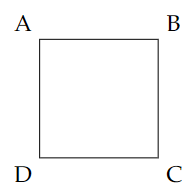
\includegraphics[scale=1]{figures/square.png}
    \end{center} 
    Let $S_4$ be the \textbf{symmetric group}, which is all 
    24 permutations of $ABCD$. Using only rotations, we can 
    only find 4 of the permutations, as shown here: 
    \begin{center}
        \begin{tabular}{c|cccc}
            $r_0$ & A & B & C & D \\ 
            $r_{90}$ & D & A & B & C \\ 
            $r_{180}$ & C & D & A & B \\ 
            $r_{270}$ & B & C & D & A
        \end{tabular}
    \end{center}
    This group can be written as $G = \set{e = r_0, r_{90}, r_{180}, r_{270}}$. 
    This group is generated by $r_{90}$ and $r_{270}$: $\langle r_{90} \rangle =  \set{r_0, r_{90}, r_{180}, r_{270}}$.
\end{example}

\begin{example}3
    Consider all symmetrices of $ABCD$: $\set{e, r_{90}, r_{180}, r_{270}, V, H, L, R}$, 
    where $V$ is a vertical reflection, $H$ is a horizontal reflection, 
    $L$ is a left diagonal reflection, \& $R$ is a right diagonal reflection. 
    \begin{center}
        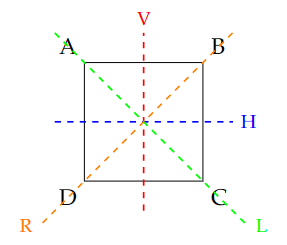
\includegraphics[scale=1]{figures/square_symmetries.png}
    \end{center}
    Let's construct a Cayley table! 
    \begin{center}
        \begin{tabular}{c|cccc|cccc}
                      & $e$       & $r_{90}$  & $r_{180}$ & $r_{270}$ & $V$       & $H$       & $L$       & $R$       \\ \hline 
            $e$       & $e$       & $r_{90}$  & $r_{180}$ & $r_{270}$ & $V$       & $H$       & $L$       & $R$       \\
            $r_{90}$  & $r_{90}$  & $r_{180}$ & $r_{270}$ & $e$       & $R$       & $L$       & $V$       & $H$       \\
            $r_{180}$ & $r_{180}$ & $r_{270}$ & $e$       & $r_{90}$  & $H$       & $V$       & $R$       & $L$       \\
            $r_{270}$ & $r_{270}$ & $e$       & $r_{90}$  & $r_{180}$ & $L$       & $R$       & $H$       & $V$       \\ \hline 
            $V$       & $V$       & $L$       & $H$       & $R$       & $e$       & $r_{180}$ & $r_{90}$  & $r_{270}$ \\
            $H$       & $H$       & $R$       & $V$       & $L$       & $r_{180}$ & $e$       & $r_{270}$ & $r_{90}$  \\
            $L$       & $L$       & $H$       & $R$       & $V$       & $r_{270}$ & $r_{90}$  & $e$       & $r_{180}$ \\
            $R$       & $R$       & $V$       & $L$       & $H$       & $r_{90}$  & $r_{270}$ & $r_{180}$ & $e$       \\
        \end{tabular}
    \end{center}
    This group is $D_4$, the dihedral group on 4 elements. We found $|D_4| = 8$ here, which generalizes to $|D_n| = 2n$. 
    It is important to note that the dihedral group is a subgroup of the set of all possible permutations. 
\end{example}

\begin{example}4
    Below is a table of decomposed operations for square $ABCD$, shown in terms of permutations: 
    \begin{center}
        \begin{tabular}{c|c}
            $e$       & $e$       \\
            $r_{90}$  & $(ADCB)$  \\
            $r_{180}$ & $(AC)(DB)$ \\
            $r_{270}$ & $(ABCD)$ \\ 
            $V$       & $(AB)(CD)$       \\
            $H$       & $(AD)(BC)$       \\
            $L$       & $(BD)$       \\
            $R$       & $(AC)$       
        \end{tabular}
    \end{center}
\end{example}